\documentclass[border=0.05cm]{standalone}
\usepackage{tikz}
\usepackage{xcolor}
\usetikzlibrary{automata, arrows.meta, positioning, calc}
\usepackage{fontspec}
\setmainfont{Arial}

% Define colors based on split-complementary scheme
% https://copic.too.com/blogs/educational/analogous-complimentary-and-split-complementary-color-schemes?srsltid=AfmBOoqZ8Nt71usioxMxPyKzjQ5vDcxs2B_imasd_wZa50UB5cZX6xCL
\definecolor{dftcolor}{RGB}{44, 163, 207}  
\definecolor{simcolor}{RGB}{237, 156, 44} 
\definecolor{expcolor}{RGB}{222, 70, 28}

% Define styles
\tikzset{
	simulated/.style={draw=simcolor!80!black, fill=simcolor!30, shape=rectangle, minimum width=2cm, minimum height=4cm, rounded corners=6pt},
	experimental/.style={draw=expcolor!80!black, fill=expcolor!40, shape=rectangle, minimum width=2cm, minimum height=4cm, rounded corners=6pt},
	synthetic/.style={draw=black, dash pattern=on 1pt off 1pt, fill=none, minimum width=0.5cm, minimum height=0.5cm, shape=rectangle}, 
	real/.style={draw=black, fill=none, minimum width=0.5cm, minimum height=0.5cm, shape=rectangle}, 
	nn/.style={draw=black, shape=circle, minimum size=0.5cm, fill=none}, 
	transfer/.style={->},
	VU/.style={thick, ->, color=simcolor},
	annotation/.style={font=\small}
}

\begin{document}
	
	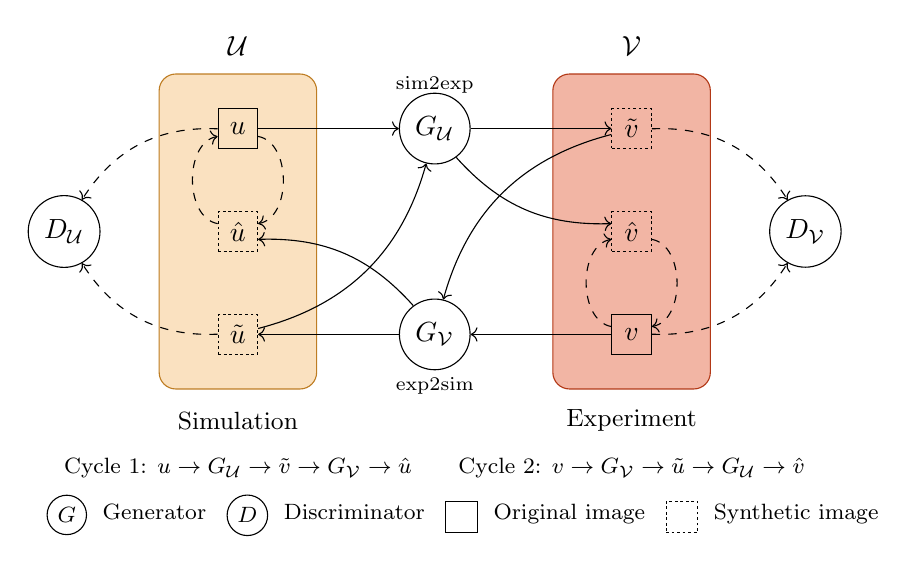
\begin{tikzpicture}[node distance = 5cm, on grid, auto]
		% U
		\node (U) [state, simulated, label={[yshift=0.1cm]above: $\mathcal{U}$}] {};
		\node[below=2.4cm of U, annotation, text=simcolor!0!black] {Simulation};
		\node (u) [real] at ($(U.north)+(0,-0.7cm)$) {$u$};
		\node (ut) [synthetic] at ($(U.south)+(0,+0.7cm)$) {$\tilde{u}$};
		\node (uh) [synthetic] at ($(u)!0.5!(ut)$)  {$\hat{u}$};
		\node at  ($(U.south)+(-0,-1cm)$) {\footnotesize
			{Cycle 1:} $u \rightarrow G_\mathcal{U} \rightarrow \tilde{v} \rightarrow G_\mathcal{V} \rightarrow \hat{u}$};
		
		% V
		\node (V) [state, right = of U, experimental, label={[yshift=0.1cm]above: $\mathcal{V}$}] {};
		\node[below=2.4cm of V, annotation, text=simcolor!0!black] {Experiment};
		\node (vt) [synthetic] at ($(V.north)+(0,-0.7cm)$)  {$\tilde{v}$};
		\node (v) [real] at ($(V.south)+(0,+0.7cm)$)  {$v$};
		\node (vh) [synthetic] at ($(v)!0.5!(vt)$) {$\hat{v}$};
		\node at  ($(V.south)+(+0,-1cm)$) {\footnotesize
			{Cycle 2:} $v \rightarrow G_\mathcal{V} \rightarrow \tilde{u} \rightarrow G_\mathcal{U}\rightarrow \hat{v}$};
		
		% G
		\node (gu) [nn] at ($(u)!0.5!(vt)$)  {$G_{\mathcal{U}}$};
		\node[above=0.55cm of gu, annotation, text=simcolor!0!black] {\scriptsize{sim2exp}};
		\node (gv) [nn] at ($(v)!0.5!(ut)$)  {$G_{\mathcal{V}}$};
		\node[below=0.65cm of gv, annotation, text=simcolor!0!black] {\scriptsize{exp2sim}};
		
		% D 
		\node (du) [nn] at ($(U.west)+(-1.2cm,0)$) {$D_{\mathcal{U}}$};
		\node (dv) [nn] at ($(V.east)+(+1.2cm,0)$) {$D_{\mathcal{V}}$};
		
		
		\path[transfer] (u) edge (gu);
		\path[transfer] (gu) edge (vt);
		\path[transfer, dashed] (vt) edge [bend left] (dv);  % adversarial loss
		\path[transfer, dashed] (v) edge [bend right] (dv); % adversarial loss
		\path[transfer] (vt) edge [bend right] (gv); % recover
		\path[transfer] (gv) edge [bend right=25] ($(uh.east)+(0,-0.1cm)$); % recover
		\path[transfer, dashed] ($(uh.west)+(0,0.1cm)$) edge [bend left=80] ($(u.west)+(0,-0.1cm)$);  % cycle consistency loss
		\path[transfer, dashed] ($(u.east)+(0,-0.1cm)$) edge [bend left=80] ($(uh.east)+(0,0.1cm)$); % cycle consistency loss
		
		\path[transfer] (v) edge (gv);
		\path[transfer] (gv) edge (ut);
		\path[transfer, dashed] (ut) edge [bend left] (du);  % adversarial loss
		\path[transfer, dashed] (u) edge [bend right] (du); % adversarial loss
		\path[transfer] (ut) edge [bend right] (gu); % recover
		\path[transfer] (gu) edge [bend right=25] ($(vh.west)+(0,+0.1cm)$); % recover
		\path[transfer, dashed] ($(vh.east)+(0,-0.1cm)$) edge [bend left=80] ($(v.east)+(0,+0.1cm)$);  % cycle consistency loss
		\path[transfer, dashed] ($(v.west)+(0,+0.1cm)$) edge [bend left=80] ($(vh.west)+(0,-0.1cm)$); % cycle consistency loss

	% Legend
	\begin{scope}[shift={([xshift=-0.4cm,yshift=-2.8cm]du.south)}]
		\node[
		anchor=north west,
		align=left,
		%draw=black,
		rounded corners,
		fill=white,
		opacity=0,
		text opacity=1,
		inner sep=2pt
		] {
			\small
			\begin{tabular}{@{}l@{}}
				%$G_\mathcal{U}$  & Style translator from $\mathcal{U}$ to $\mathcal{V}$ \raisebox{-0.4ex}{\includegraphics[width=0.4cm]{nn.pdf}}& \\
				%$G_\mathcal{V}$  & Style translator from $\mathcal{V}$ to $\mathcal{U}$ \raisebox{-0.4ex}{\includegraphics[width=0.4cm]{nn.pdf}}& \\
				%$D_\mathcal{U}$  & Discriminator in domain $\mathcal{U}$  \raisebox{-0.4ex}{\includegraphics[width=0.4cm]{nn.pdf}}& \\
				%$D_\mathcal{V}$  & Discriminator in domain $\mathcal{V}$  \raisebox{-0.4ex}{\includegraphics[width=0.4cm]{nn.pdf}}& \\

				%$u$  & Simulated AFM image& \\
				%$v$  & Experimental AFM image& \\
				%$\hat{u}$ & $u \rightarrow G_\mathcal{U} \rightarrow \tilde{v} \rightarrow G_\mathcal{V}$ $\rightarrow \hat{u}$&\\
				%$\hat{v}$ & $v \rightarrow G_\mathcal{V} \rightarrow \tilde{u} \rightarrow G_\mathcal{U}$ $\rightarrow \hat{v}$&\\
			\footnotesize{
      		\raisebox{0ex}{\tikz[baseline=-2ex] \node(N) [nn, minimum size=0.5cm] {$G$};} \hspace{0em} Generator
			\hspace{0.2em}
			\tikz[baseline=-2ex] \node(D) [nn, minimum size=0.5cm] {$D$}; \hspace{0em} Discriminator
			\hspace{0.2em}
			\tikz[baseline=-2.0ex] \node(R) [real, rounded corners=0pt, minimum size=0.4cm] {}; \hspace{0em} Original image
			\hspace{0.2em}
			\tikz[baseline=-2.0ex] \node(T) [synthetic, rounded corners=0pt, minimum size=0.4cm] {}; \hspace{0em} Synthetic image}\\
			\end{tabular}
		};
	\end{scope}
	\end{tikzpicture}
	
\end{document}